\newcommand{\projectName}{Az EGTIB}

\chapter{\projectName{} bemutatása}

\projectName{} projekt célja egy olyan felhasználóbarát felület létrehozása, mely lehetőséget teremt a daganatos sejtek játékelméleti modellezésére és szimulációjára, a szimulációs eredmények megjelenítésére illetve ezeknek valamilyen szintű mentésére is. Ezért született meg, a mai trendeket figyelembe véve, egy kliens-szerver architektúrán alapuló webalkalmazás, mely részben az \cite{archetti2016cooperation}-ben megjelent modellt implementálja, és ahhoz új funkcionalitásokat is hozzáad.

\begin{figure}[ht!]
	\centering
	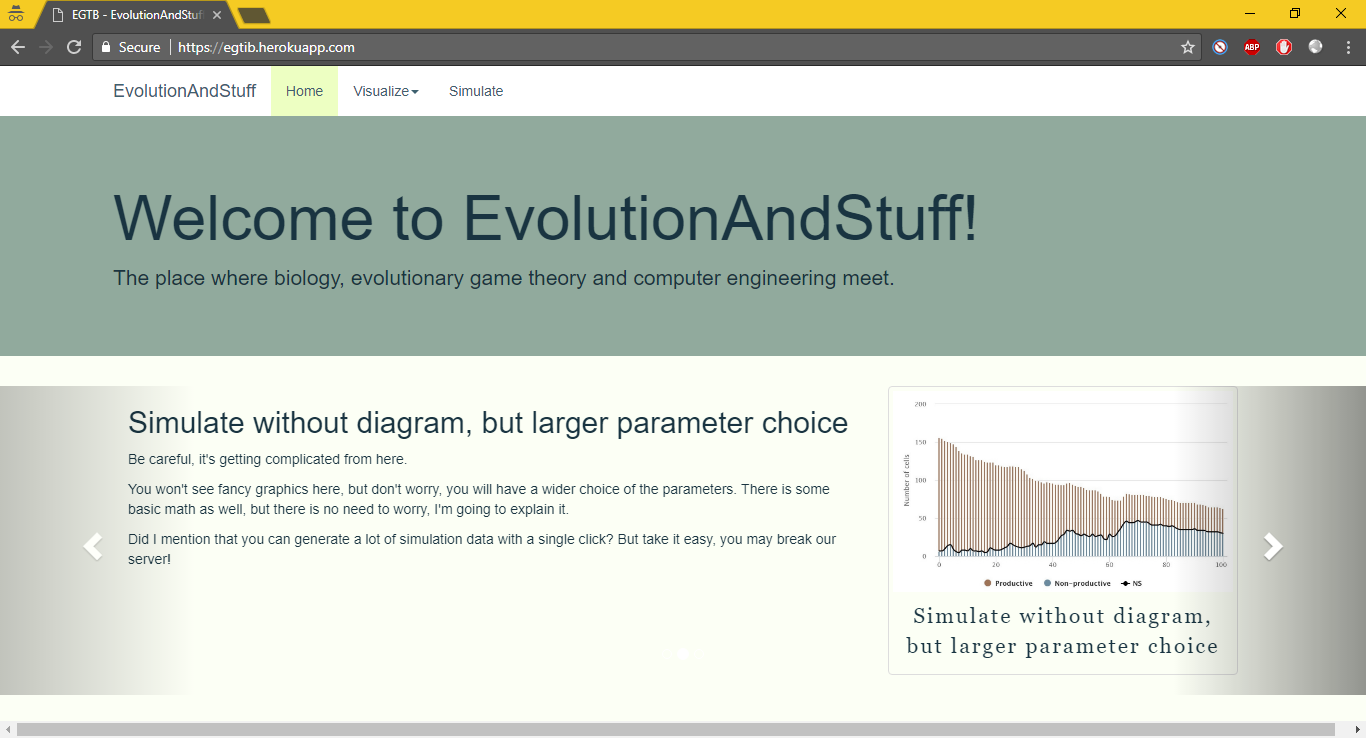
\includegraphics[width=0.98\linewidth]{images/welcomePage}
	\caption{Főoldal}
	\label{fig:welcomePage}
\end{figure}

\section{Funkcionalitások}

Az alkalmazásunkat egy főoldalra, valamint funkcionalitás szerint, három fő komponensre oszthatjuk:

\paragraph{Üdvözlő oldal}- ezen az oldalon kaptak helyet az általános jellegű információk és egy boostrap carousel, amellyel az alkalmazás mindegyik fő komponense rövid és humoros szövegekkel van bemutatva, valamint egy kép amely tovább visz az adott oldalra (\ref{fig:welcomePage} ábra)

\paragraph{Vizualizáció}- a vizualizációs oldalra tévedve (\ref{fig:VisualizationDiagram}), a felhasználó elég sok újdonsággal találja magát szemben. Az legszembeötlőbb egy színes pöttyökkel teli rajz lesz, ami a Voronoi diagram. Itt a kooperáló és defektáló sejtek narancssárga illetve sötétbarna színben vannak reprezentálva. A képernyő második legnagyobb részét a diagramtól balra elhelyezkedő paraméterlista tölti ki. Itt a következő paramétereket lehet állítgatni, amelyek a szimulációt befolyásolják:
\begin{itemize}
	\item kezdeti populáció mérete
	\item defektálók aránya 
	\item generáció szám (szimuláció hossza)
	\item kooperáló sejtek termelési költsége 
	\item diffúziós távolság mérete
	\item akarja-e a felhasználó, hogy a sejtek osztódásra legyenek képesek
\end{itemize}

\begin{figure}[ht!]
	\centering
	\captionsetup{justification=centering}
	\begin{tabular}{cc}
		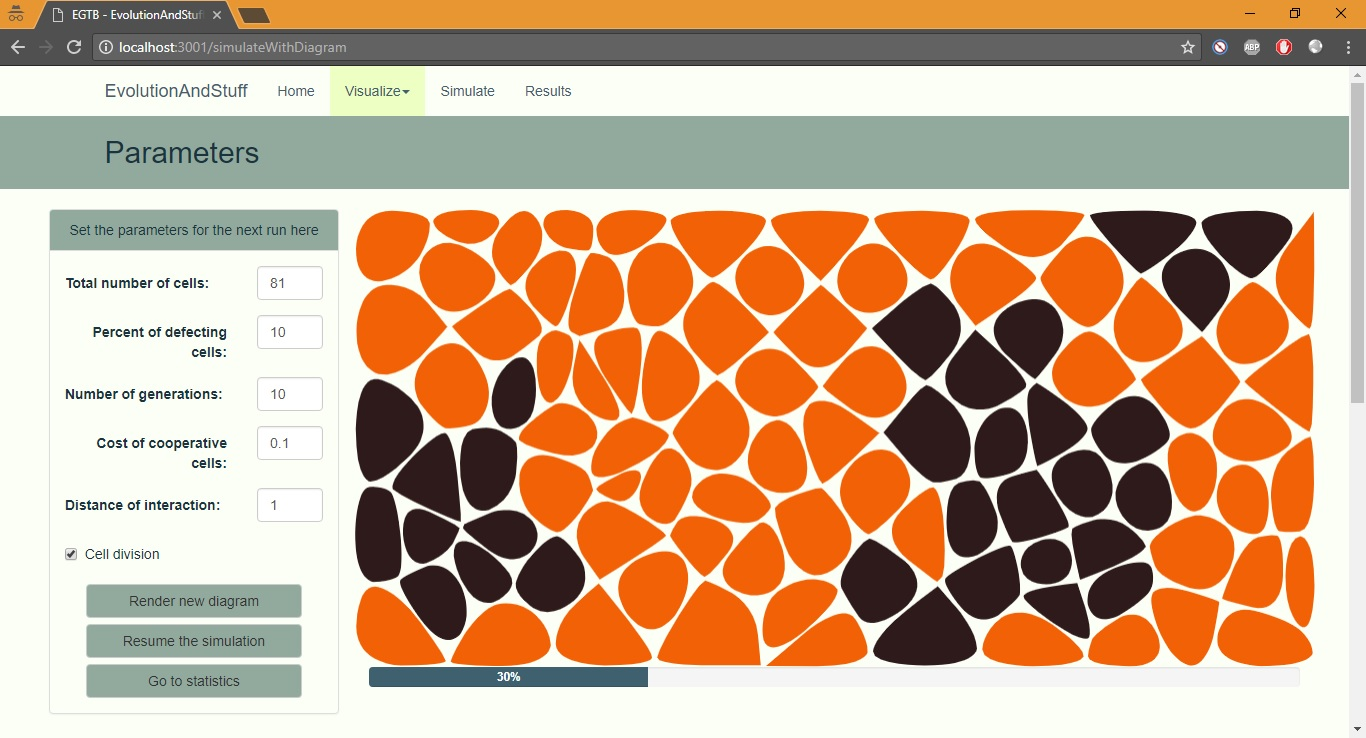
\includegraphics[width=0.47\linewidth]{images/EGTIB}
		&
		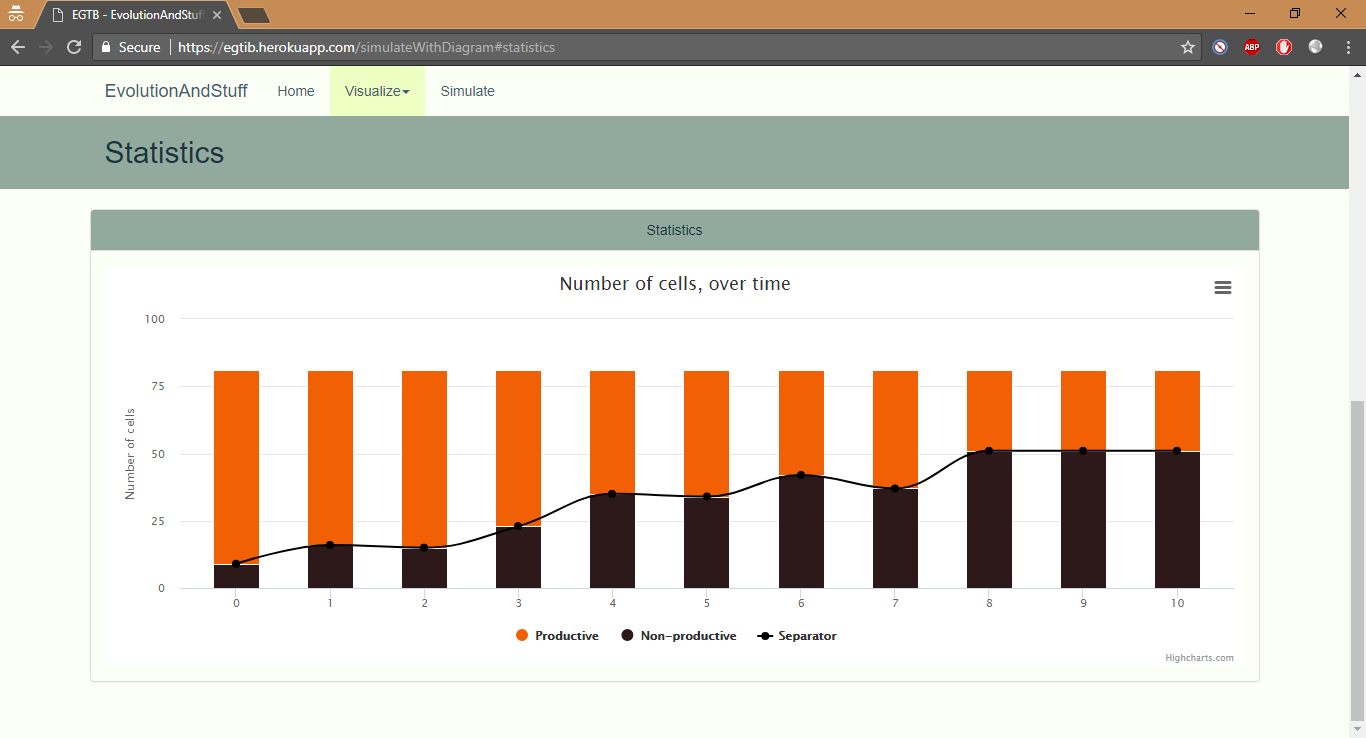
\includegraphics[width=0.47\linewidth]{images/VisualizationDiagram}
	\end{tabular}
	\caption{Bal: vizualizációs oldal, Voronoi diagram, paraméterek. Jobb: a populáció változása generációnként adott paraméterekre}	
	\label{fig:VisualizationDiagram}
\end{figure}

A paraméterlista alatt található az új Voronoi diagramot generáló gomb is. Erre szükség van, mivel minden paraméter változásnál a Voronoi diagramot újra kirajzolni túlságosan költséges lenne és nagyon belassítani az oldalt, ezzel rontva a felhasználói élményt. A szimuláció elindításáért felelős gomb is itt kapott helyet, amely a szimuláció során megállít és folytat gombra cserélődik, attól függően, hogy a szimulációt megállítjuk-e. Amennyiben a felhasználó lusta lenne letekerni az oldal aljára, elhelyeztünk számára egy statisztikához ugró gombot is. Ha a felhasználó egy kicsikét leleményes, akkor rájön arra is, hogy amennyiben megállítja a szimuláció lejátszását, a Voronoi diagram alatt elhelyezett progress bar segítségével tekergetheti a szimulációt, pont úgy mint egy filmet.
Megszorítása ezen oldalnak, hogy 500 sejtnél többet nem lehet vele kirajzoltatni, illetve szimulálni, mert annak kirajzolása túlságosan költséges, a felhasználó csak annyit érzékelne, hogy az oldal megfagyott.

\paragraph{Szimuláció}- erre az oldalra (\ref{fig:SimulationFunctionDiagrams} ábra) kerültek az átlag felhasználónak nem sokat mondó paraméterek, valamint a sejtek száma is csak annyira korlátozott, amennyit a szerver képes szimulálni (max. 2000 sejt). Első szembeötlő eltérés a vizualizációs oldalhoz képest az, hogy itt már nincs Voronoi diagram, többek között ezért sincs annyira megkötve a sejtek maximális száma. Itt már nem kerül kirajzolásra a szimuláció, de természetesen a statisztikás grafikon itt is megjelenik. A felhasználó belenyúlhat az alábbi paraméterekbe is ezen az oldalon:
\begin{itemize}
	\item a V függvény meredeksége
	\item a V függvény áthajlási pontjának helye
	\item a gradiens alakja
	\item a gradiens meredeksége az áthajlási pontban
\end{itemize}
Mivel ezek csak nyers számok, ezért jó ötletnek gondoltuk azt, hogy a  V (\ref{eq:payoffGradient} képlet) és g (\ref{eq:diffGradient} képlet) függvényeket jelenítsük meg. Ezen grafikonok elhelyezése egyszerű volt, hisz a Voronoi diagram helyét vették át. Itt a paraméterek változtatása interaktív, ami annyit jelent, hogy amint a paraméter értékét átírjuk, úgy a grafikon is annak megfelelően változik.

Eléggé repetitívvé válik a felhasználó munkája amennyiben hasonló paraméterekre szeretne szimulációkat végezni, így az a lehetősége is megvan, hogy bizonyos paramétereket nem csak számként, hanem az alábbi formában is megadjon: 0.1:0.1:1. Ez azt jelenti, hogy 0.1-től indulva 0.1-esével egészen 1-ig minden értéket felvesz az adott paraméter és azon szimulációkat kéri le a szervertől.

\begin{figure}[ht!]
	\centering
	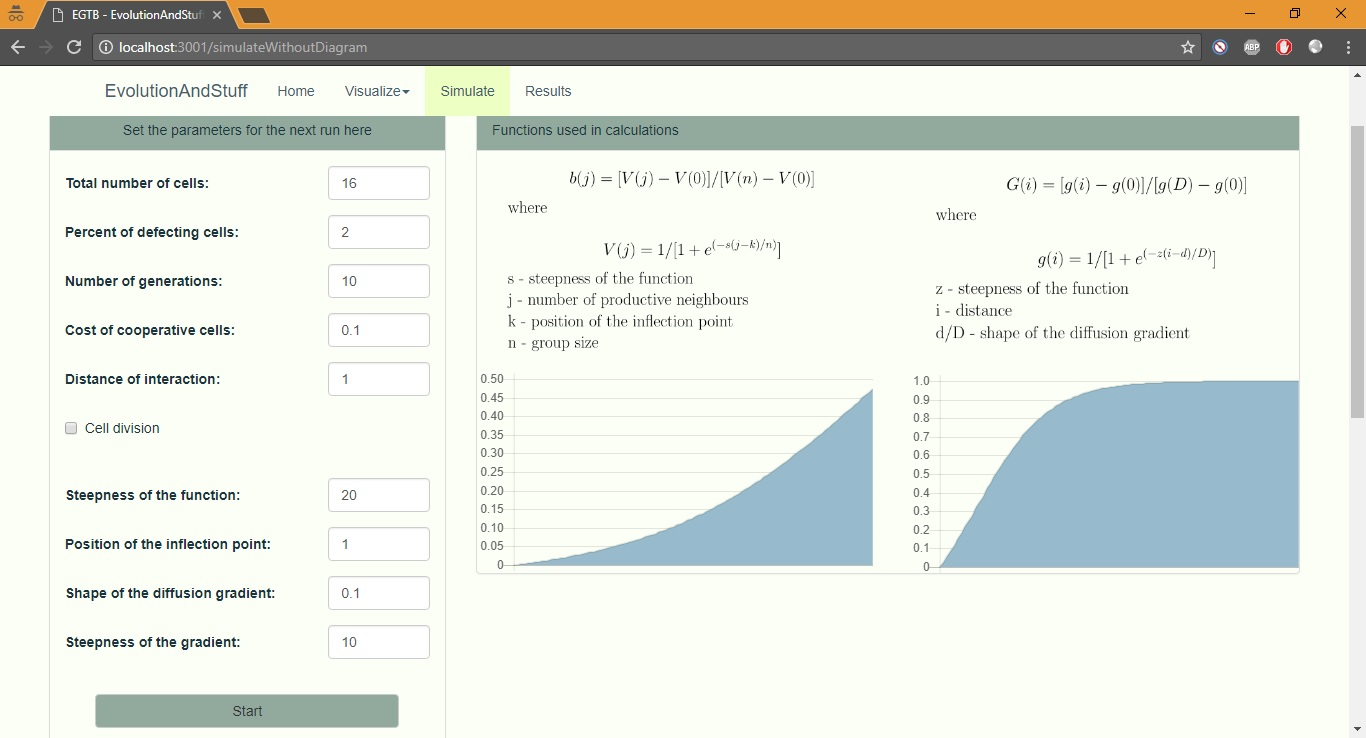
\includegraphics[width=90mm]{images/SimulationFunctionDiagrams}
	\caption{A V és g függvények alakja adott paraméterekre}
	\label{fig:SimulationFunctionDiagrams}
\end{figure}


\paragraph{Eredmények}- kezdetben már azzal is megelégedtünk, ha egy szimulációt képesek voltunk megjeleníteni, viszont egy idő után azt vettük észre, hogy milyen jó lenne ha ezeket nem kellene mindig újra és újra generálni. Így született meg az eredményeket tartalmazó rész mely megjeleníti az oldalon futtatott szimulációkat egy error bar segítségével. Mivel a bemeneti paraméterek eléggé változatosak lehetnek, így valamilyen szinten ezen adatokat a megjelenítés során szűrni kell. Ezért a felhasználó ezt köteles is megtenni mielőtt az eredményeket megtekintené, az alábbiak szerint:
\begin{itemize}
	\item defektáló sejtek aránya
	\item kooperálási költség 
	\item interakció távolsága
\end{itemize}
Ezen adatok megadása után, az összes olyan szimuláció mely kielégíti a feltételeket egyesítve lesz egy grafikonon (\ref{fig:SimulationResults} ábra).

\begin{figure}[ht!]
	\centering
	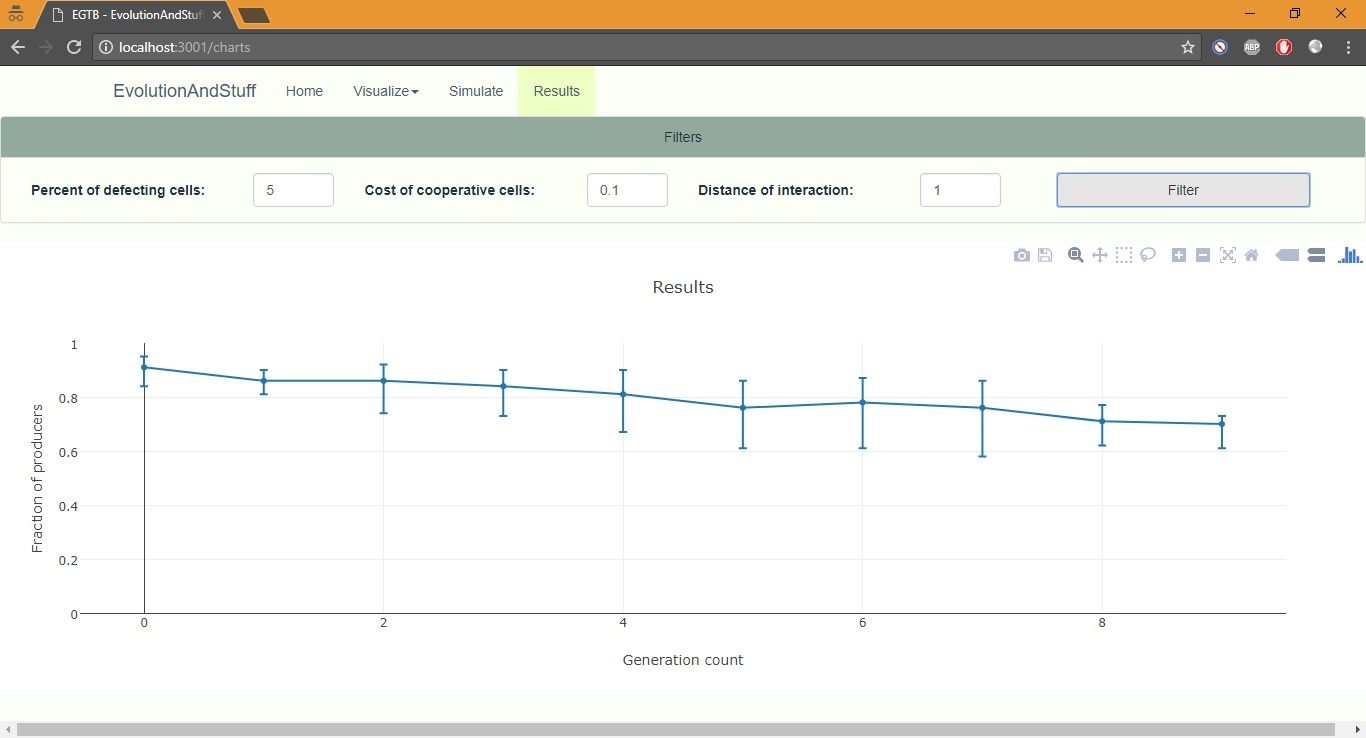
\includegraphics[width=90mm]{images/SimulationResults}
	\caption{Eddigi szimulációk eredményei}
	\label{fig:SimulationResults}
\end{figure}


\section{Felhasznált technológiák}

Már a projekt kezdetekor biztosak voltunk benne, hogy egy könnyen és bárki által elérhető alkalmazásra lesz szükség, így nem volt kérdéses az, hogy webes felületet akarunk. Ezután már csak az volt a kérdéses, hogy számunkra milyen környezet lenne a legkényelmesebb, amely ha szükség van rá könnyen skálázható is. Végül a \textbf{NodeJS}-re (\cite{soft:node}) esett a választásunk, hiszen ez egy egyszerű felület skálázható hálózati alkalmazások írására, valamint egy nagyon egyszerű és elterjedt nyelvet használ, a JavasSriptet. Keretrendszernek a sokak által ismert és használt \textbf{ExpressJS}-t (\cite{soft:express}) választottuk.

Tehát a szoftver egy szerverből és egy kliensből áll, melyek közötti kommunikáció a már jól megszokott HTTP-vel folyik. A fejlesztés során bizonyos szimulációs adatok JSON-beli küldözgetése túl nagy feladatnak bizonyult, így ezek átvitelét \textbf{WebSocket} segítségével oldottuk meg. Azt is jó tudni, hogy a szerver oldalon folyik az erőforrás igényes számítások nagy része.

Említettük, hogy \textbf{Voronoi} diagramokkal ábrázoljuk a sejteket, így szükségünk volt egy Voronoi modulra is (\cite{soft:voronoiModule}). Ez a modul egy JavaScript implementációja Steven J. Fortune algoritmusának, mely hatékonyon dolgozik Voronoi diagramokkal, viszont csak az adatszerkezettel foglalkozik, nem képes ki is rajzolni azt.

Webalkalmazásról lévén szó szükség van egy adatbázisra is ahol a szesszió adatokat el lehet tárolni, ez a \textbf{MongoDB} (\cite{soft:mongodb}). Továbbá a szimulációs eredmények lementése is ide történik, és természetesen az eredmények oldal kigenerálása során is innen vesszük ki az adatokat. Emeljük ki azt a tényt, hogy a MongoDB sokat könnyített a munkánkon az adatok lementését illetően. Adataink JavaScript objektumokként vannak reprezentálva és köszönhetően az adatbázisnak, nem volt szükségünk semmilyen tervezésre, egyszerűen le lehet ilyen struktúrában lévő adatokat menteni, majd ezek lekérése is könnyen megvalósítható.

\begin{figure}[ht!]
	\centering
	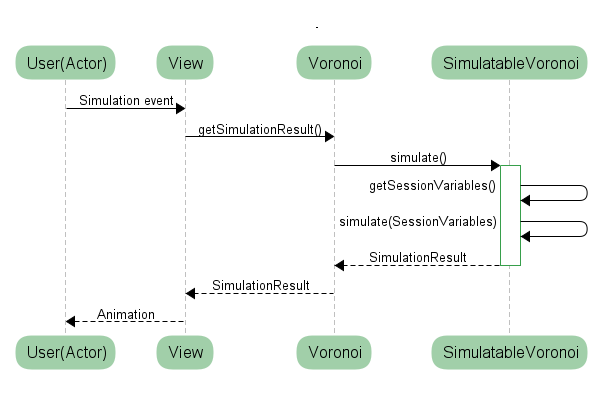
\includegraphics[width=\linewidth]{images/SimulationProcess}
	\caption{Szekvencia diagram. A szimulálási folyamat lépései}
	\label{fig:SimulationProcess}
\end{figure}


Kliens oldalon a technológiák felhozatala eléggé változatos. Először is egy weboldal jól kell kinézzen és ezen feladatot a \textbf{Bootstrap} (\cite{soft:bootstrap}) keretrendszer tökéletesen ki is elégíti. Dinamikus oldalt lehet vele létrehozni, bármilyen eszközt együttesen lehet kezelni vele, nem csak desktopon de mobil eszközökön is jól néz ki az oldal. Kezdetben kliens oldalon nem nagyon volt bármiféle struktúra a JavaScriptben és elég hamar rá is jöttünk, hogy ez egy hatalmas probléma, a kód elég hamar átláthatatlan lett. Ezért átálltunk \textbf{AngularJS}-re (\cite{soft:angular}), mellyel már sokkal olvashatóbb kódot sikerült létrehoznunk, egyszerűbbé tette a kód bővítését is és az oldal dinamikussága is nőtt (pl. megjelentek az alertek). A Voronoi diagram megjelenítéséért a \textbf{Paper.js} (\cite{soft:paper}) a felelős, valamint itt is jelen van a Voronoi adatszerkezetet feldolgozó modul (\cite{soft:voronoiModule}). A grafikonok kirajzolására több keretrendszert is használunk. Ez azért van, mert ismertünk már egyet ami az adott feladatot kielégítette, viszont a későbbiekben új típusú diagramok jöttek be, melyekhez, mint kiderült, új keretrendszerre volt szükségünk. Így alakult, hogy a Voronoi diagram alatti grafikont a \textbf{Highcharts} (\cite{soft:highcharts}) segítségével, a V és g függvényeket (\ref{fig:SimulationFunctionDiagrams}) az AngularJS grafikonjaival, míg az error bart (\ref{fig:SimulationResults}) a \textbf{Plotly.js} (\cite{soft:plotly}) segítségével rajzoltuk ki.

Mivel ez az egész egy webalkalmazás szükségünk volt egy szerverre, ahova ezt kitelepíthetjük. Míg régen ez egy saját szerverre telepítették mely egy statikus IP címmel rendelkezett, addig mára már sokkal könnyebb ha ezt inkább egy felhőbe rakjuk. Több ingyenesen használható felhő is létezik már, a mi választásunk a \textbf{Heroku} lett (az alábbi linken érhető el az alkalmazásunk: \url{https://egtib.herokuapp.com/}). A Heroku egy PaaS típusú felhőszolgáltató, ami annyit jelent, hogy platformot és kész szolgáltatásokat nyújt. Elég volt csak azt megmondani, hogy egy NodeJS alapú szervert akarunk üzemeltetni, ahhoz kiválasztottunk egy akármilyen adatbázist, és már kész is. Természetesen senki sem szereti a kitelepítést kézzel elvégezni, ezért, és persze még sok más hasznos funkcióért is, automatizáltuk a fejlesztést a \textbf{TravisCI} (\cite{soft:travis}) segítségével. A TravisCI egy folytonos integrációs platform, mely könnyen összeköthető github projektekkel, és minden egyes alkalmazás frissítéskor képes előre megadott parancsokat elvégezni. Továbbá ha az alkalmazásunkat egy \textbf{Docker}-be (\cite{soft:docker}) rakjuk, akkor biztosíthatjuk azt, hogy bárhova is kerül az alkalmazásunk, mindig ugyanazon körülmények között fog futni.

Semmilyen kódot nem adhatunk ki a kezünkből, ha annak minősége nincs valahogyan biztosítva. Ezt a minőséget tesztekkel lehet valamilyen szinten biztosítani, amit is megpróbáltunk. Köszönhetően a TravisCI-nak a tesztelés beépítése a fejlesztési folyamatba könnyen ment. Minden egyes új verzió felkerülésekor a github repositoryba, a Travis lefuttatja a teszteket és jelezi, hogy ezek között van-e olyan amely megbukott, illetve rak egy zöld pipát ha mind átment. A unit tesztjeink a \textbf{Mocha} (\cite{soft:mocha}), míg az E2E tesztjeink a \textbf{TestCafe} (\cite{soft:testcafe}) keretrendszerekben íródtak. Ezek közül kiemeljük a TestCafet, mert ez egy olyan keretrendszer melynél nincs szükség böngésző driverre, egyenesen egy előre telepített böngészőt használ, illetve fel lehet venni vele kattintásokat, azaz ki lehet vele generálni a tesztesetet és nem kell hozzá kódot írni.

\begin{figure}[ht!]
	\centering
	\includegraphics[width=\linewidth]{images/Architecture}
	\caption{A projekt architektúrája}
	\label{fig:Architecture}
\end{figure}
